\iffalse
\let\negmedspace\undefined
\let\negthickspace\undefined
\documentclass[journal,12pt,onecolumn]{IEEEtran}
\usepackage{cite}
\usepackage{amsmath,amssymb,amsfonts,amsthm}
%\usepackage{algorithmic}
\usepackage{graphicx}
\usepackage{textcomp}
\usepackage{array}
\usepackage{xcolor}
\usepackage{txfonts}
\usepackage{listings}
\usepackage{enumitem}
\usepackage{mathtools}
\usepackage{gensymb}
\usepackage[breaklinks=true]{hyperref}
\usepackage{tkz-euclide} % loads  TikZ and tkz-base
\usepackage{listings}
\usepackage{float}
\usepackage{bm}
\usepackage{tikz}
\usetikzlibrary{decorations.markings}



\newtheorem{theorem}{Theorem}[section]
\newtheorem{problem}{Problem}
\newtheorem{proposition}{Proposition}[section]
\newtheorem{lemma}{Lemma}[section]
\newtheorem{corollary}[theorem]{Corollary}
\newtheorem{example}{Example}[section]
\newtheorem{definition}[problem]{Definition}
%\newtheorem{thm}{Theorem}[section] 
%\newtheorem{defn}[thm]{Definition}
%\newtheorem{algorithm}{Algorithm}[section]
%\newtheorem{cor}{Corollary}
\newcommand{\BEQA}{\begin{eqnarray}}
\newcommand{\EEQA}{\end{eqnarray}}
\newcommand{\define}{\stackrel{\triangle}{=}}
\theoremstyle{remark}
\newtheorem{rem}{Remark}
%\bibliographystyle{ieeetr}
\begin{document}
%
\providecommand{\pr}[1]{\ensuremath{\Pr\left(#1\right)}}
\providecommand{\prt}[2]{\ensuremath{p_{#1}^{\left(#2\right)} }}        % own macro for this question
\providecommand{\qfunc}[1]{\ensuremath{Q\left(#1\right)}}
\providecommand{\sbrak}[1]{\ensuremath{{}\left[#1\right]}}
\providecommand{\lsbrak}[1]{\ensuremath{{}\left[#1\right.}}
\providecommand{\rsbrak}[1]{\ensuremath{{}\left.#1\right]}}
\providecommand{\brak}[1]{\ensuremath{\left(#1\right)}}
\providecommand{\lbrak}[1]{\ensuremath{\left(#1\right.}}
\providecommand{\rbrak}[1]{\ensuremath{\left.#1\right)}}
\providecommand{\cbrak}[1]{\ensuremath{\left\{#1\right\}}}
\providecommand{\lcbrak}[1]{\ensuremath{\left\{#1\right.}}
\providecommand{\rcbrak}[1]{\ensuremath{\left.#1\right\}}}
\newcommand{\sgn}{\mathop{\mathrm{sgn}}}
\providecommand{\abs}[1]{\left\vert#1\right\vert}
\providecommand{\res}[1]{\Res\displaylimits_{#1}} 
\providecommand{\norm}[1]{\left\lVert#1\right\rVert}
%\providecommand{\norm}[1]{\lVert#1\rVert}
\providecommand{\mtx}[1]{\mathbf{#1}}
\providecommand{\mean}[1]{E\left[ #1 \right]}
\providecommand{\cond}[2]{#1\middle|#2}
\providecommand{\fourier}{\overset{\mathcal{F}}{ \rightleftharpoons}}
\newenvironment{amatrix}[1]{%
  \left(\begin{array}{@{}*{#1}{c}|c@{}}
}{%
  \end{array}\right)
}
%\providecommand{\hilbert}{\overset{\mathcal{H}}{ \rightleftharpoons}}
%\providecommand{\system}{\overset{\mathcal{H}}{ \longleftrightarrow}}
	%\newcommand{\solution}[2]{\textbf{Solution:}{#1}}
\newcommand{\solution}{\noindent \textbf{Solution: }}
\newcommand{\cosec}{\,\text{cosec}\,}
\providecommand{\dec}[2]{\ensuremath{\overset{#1}{\underset{#2}{\gtrless}}}}
\newcommand{\myvec}[1]{\ensuremath{\begin{pmatrix}#1\end{pmatrix}}}
\newcommand{\mydet}[1]{\ensuremath{\begin{vmatrix}#1\end{vmatrix}}}
\newcommand{\myaugvec}[2]{\ensuremath{\begin{amatrix}{#1}#2\end{amatrix}}}
\providecommand{\rank}{\text{rank}}
\providecommand{\pr}[1]{\ensuremath{\Pr\left(#1\right)}}
\providecommand{\qfunc}[1]{\ensuremath{Q\left(#1\right)}}
	\newcommand*{\permcomb}[4][0mu]{{{}^{#3}\mkern#1#2_{#4}}}
\newcommand*{\perm}[1][-3mu]{\permcomb[#1]{P}}
\newcommand*{\comb}[1][-1mu]{\permcomb[#1]{C}}
\providecommand{\qfunc}[1]{\ensuremath{Q\left(#1\right)}}
\providecommand{\gauss}[2]{\mathcal{N}\ensuremath{\left(#1,#2\right)}}
\providecommand{\diff}[2]{\ensuremath{\frac{d{#1}}{d{#2}}}}
\providecommand{\myceil}[1]{\left \lceil #1 \right \rceil }
\newcommand\figref{Fig.~\ref}
\newcommand\tabref{Table~\ref}
\newcommand{\sinc}{\,\text{sinc}\,}
\newcommand{\rect}{\,\text{rect}\,}
%%
%	%\newcommand{\solution}[2]{\textbf{Solution:}{#1}}
%\newcommand{\solution}{\noindent \textbf{Solution: }}
%\newcommand{\cosec}{\,\text{cosec}\,}
%\numberwithin{equation}{section}
%\numberwithin{equation}{subsection}
%\numberwithin{problem}{section}
%\numberwithin{definition}{section}
%\makeatletter
%\@addtoreset{figure}{problem}
%\makeatother

%\let\StandardTheFigure\thefigure
\let\vec\mathbf

\bibliographystyle{IEEEtran}





\bigskip

%\renewcommand{\thefigure}{\theenumi}
%\renewcommand{\thetable}{\theenumi}
%\renewcommand{\theequation}{\theenumi}

Q: Figures correspond to two circular motions. The radius of the circle, the period of revolution, the initial position and the sense of revolution(i.e. clockwise or anti-clockwise) are indicated on each figure. Obtain the corresponding simple harmonic motions of the x-projections of the radius vector of resolving particle P in each case.

\begin{tikzpicture}
	\draw[cyan, line width=1pt] (3,5) circle [radius=2];
	\draw[postaction={decorate,decoration={markings,mark=at position 0.75 with {\arrow[scale=3]{<}}}}] (3,5) circle [radius=2];
    \draw[->] (1,5) -- (6,5) node[right] {$x$}; % X-axis with arrow and label
    \draw[->] (3,2) -- (3,8) node[above] {$y$}; % Y-axis with arrow and label
    \node[right] at (0,5) {$T=2s$}; % Variable at the end of the x-axis
    \node[above] at (3,2) {P($t=0$)}; % Parameter at the end of the y-axis
	\node[below right] at (2,5) {3 cm}; % Radius label next to the x-axis
	 \draw (3,0) node[below] {(a)}; % Label (a)
    
    % Circle (b)
    \draw[cyan, line width=1pt] (12,5) circle [radius=3]; % Circumference in red with a 1pt line width
	\draw[postaction={decorate,decoration={markings,mark=at position 0.75 with {\arrow[scale=3]{>}}}}] (12,5) circle [radius=3];
    \draw[->] (8,5) -- (16,5) node[right]{$x$}; % X-axis with arrow and label
	\draw[->] (12,0) -- (12,10) node[above]{$y$}; % Y-axis with arrow and label
	\node[right] at (7,5) {P($t=0$)}; % Variable at the end of the x-axis
 11     \node[above] at (15,5) {$T=4s$}; %Parameter at the end of the x-axis
	\node[below right] at (10,5){2m}; % Radius label next to the x-axis
	\draw (12,0) node[below]{(b)};% Label (b)

\end{tikzpicture}





\solution
\fi
\begin{table}[H]
\centering
\begin{tabular}{|c|c|c|c|}
        \hline
        \textbf{Parameter} & \textbf{Value(a)} & \textbf{Value(b)} & \textbf{Description}\\
        \hline
	Radius(r) & $3\text{cm}$ & $2\text{m}$ & Radius of each circle \\
        \hline
	Time Period(T) & $2\text{s}$ & $4\text{s}$ & Time period \\
	\hline
	Sense & clockwise & anti-clockwise & Indicated by arrow\\
	\hline
	Initial Phase$(\phi)$ & $\frac{\pi}{2}$ & $\pi$ & Initial angle with x-axis\\
	\hline
\end{tabular}
\caption{Input parameters table}
\label{tab:11.14.11}

\end{table}
Given $\myvec{r}$ as radius vector making angle $\theta$ with positive x-axis, its x-projection = $\myvec{r}\cos{\theta}$ \\
\begin{enumerate}[label=\alph*.]
\item At $t=0$, the radius vector makes an angle $\frac{\pi}{2}$ with the positive x-axis, $\phi = \frac{\pi}{2}$, \\
From \tabref{tab:11.14.11}, equation of x-projection of radius:
\begin{align}
x(t) &= r\cos\brak{\frac{2\pi}{T}t + \phi} \\
	&= 3\cos\brak{\frac{2\pi}{2}t + \frac{\pi}{2}} \\
	&= -3\sin\brak{\pi{t}}\text{cm}
\end{align}
\begin{figure}[ht]
	\centering
	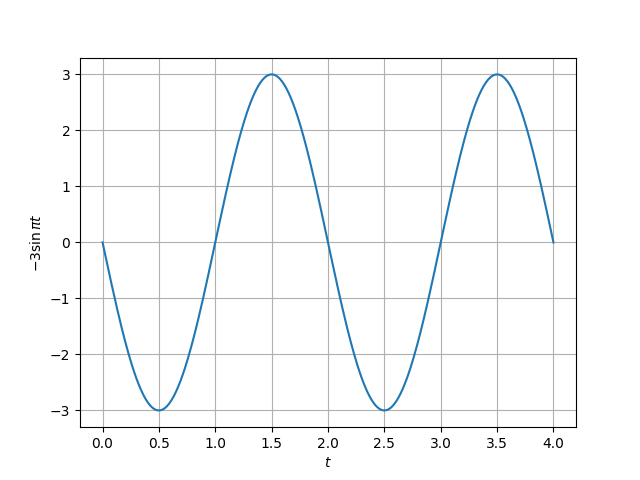
\includegraphics[width=0.8\textwidth]{ncert-physics/11/14/11/figs/fig1.png}
\end{figure}
\item Similarly, \\
At $t=0$, radius vector makes an angle $\pi$ with x-axis in anti-clockwise direction, $\phi = \pi$,
\begin{align}
x(t) &= r\cos\brak{\frac{2\pi}{T}t + \phi} \\
	&= 2\cos\brak{\frac{2\pi}{4}t + \pi} \\
	&= -2\cos\brak{\frac{\pi}{2}t}\text{m}
\end{align}
\begin{figure}[ht]
	\centering
	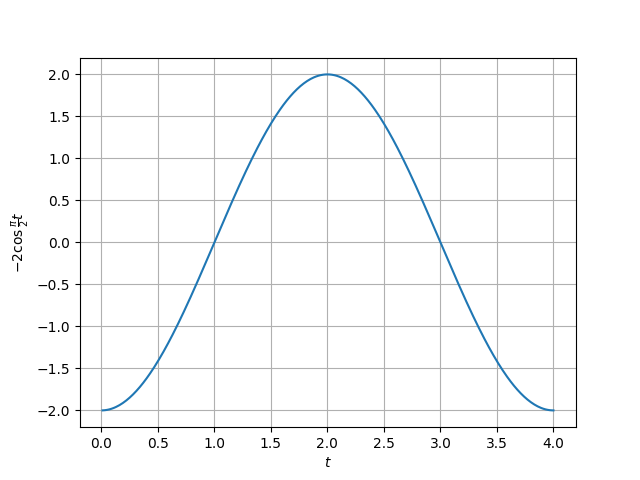
\includegraphics[width=0.8\textwidth]{ncert-physics/11/14/11/figs/fig2.png}
\end{figure}
	\end{enumerate}
	
%\end{document}
